% This is samplepaper.tex, a sample chapter demonstrating the
% LLNCS macro package for Springer Computer Science proceedings;
% Version 2.20 of 2017/10/04
%
\documentclass[runningheads]{llncs}
%
\usepackage{graphicx}
\usepackage{amsmath}
% Used for displaying a sample figure. If possible, figure files should
% be included in EPS format.
%
% If you use the hyperref package, please uncomment the following line
% to display URLs in blue roman font according to Springer's eBook style:
% \renewcommand\UrlFont{\color{blue}\rmfamily}

\begin{document}
%
\title{Using Logistic Regression to Identify 'Troll' User Intentions}
%
%\titlerunning{Abbreviated paper title}
% If the paper title is too long for the running head, you can set
% an abbreviated paper title here
%
%
\authorrunning{A. Panagos}
% First names are abbreviated in the running head.
% If there are more than two authors, 'et al.' is used.
%
\author{Arryn G.H. Panagos}

\institute{Department of Biostatistics \\ Univeristy of North Carolina-Chapel Hill, Chapel Hill, NC \\
\email{arryn@live.unc.edu}}

%
\maketitle              % typeset the header of the contribution
%
\begin{abstract}
 Given the surge in social media use, there has been an ever-increasing interest in 'trollish' behavior and its effect on other users. There are questions as to what trolls are trying to affect and how they are achieving their goals. We were interested in using supervised learning to identify troll characteristics. Using TF-IDF bag-of-words with the logistic regression, we were able to identify words characterizing trolls/non-trolls. However, the difference between the raw TF-IDF and weighted post-training word frequency was mostly negligible. However, this outcome does increase the confidence that the raw TF-IDF high-value words do paint a good picture of troll intentions. The word intentions were in alignment with western narratives.
\
\keywords{IRA  \and troll tweets \and logistic regression \and twitter}
\end{abstract}
%
%
%
\section{Social Media Information Warfare}
\subsection{IRA Tweet Data and TF-IDF}

\begin{figure}
\centering
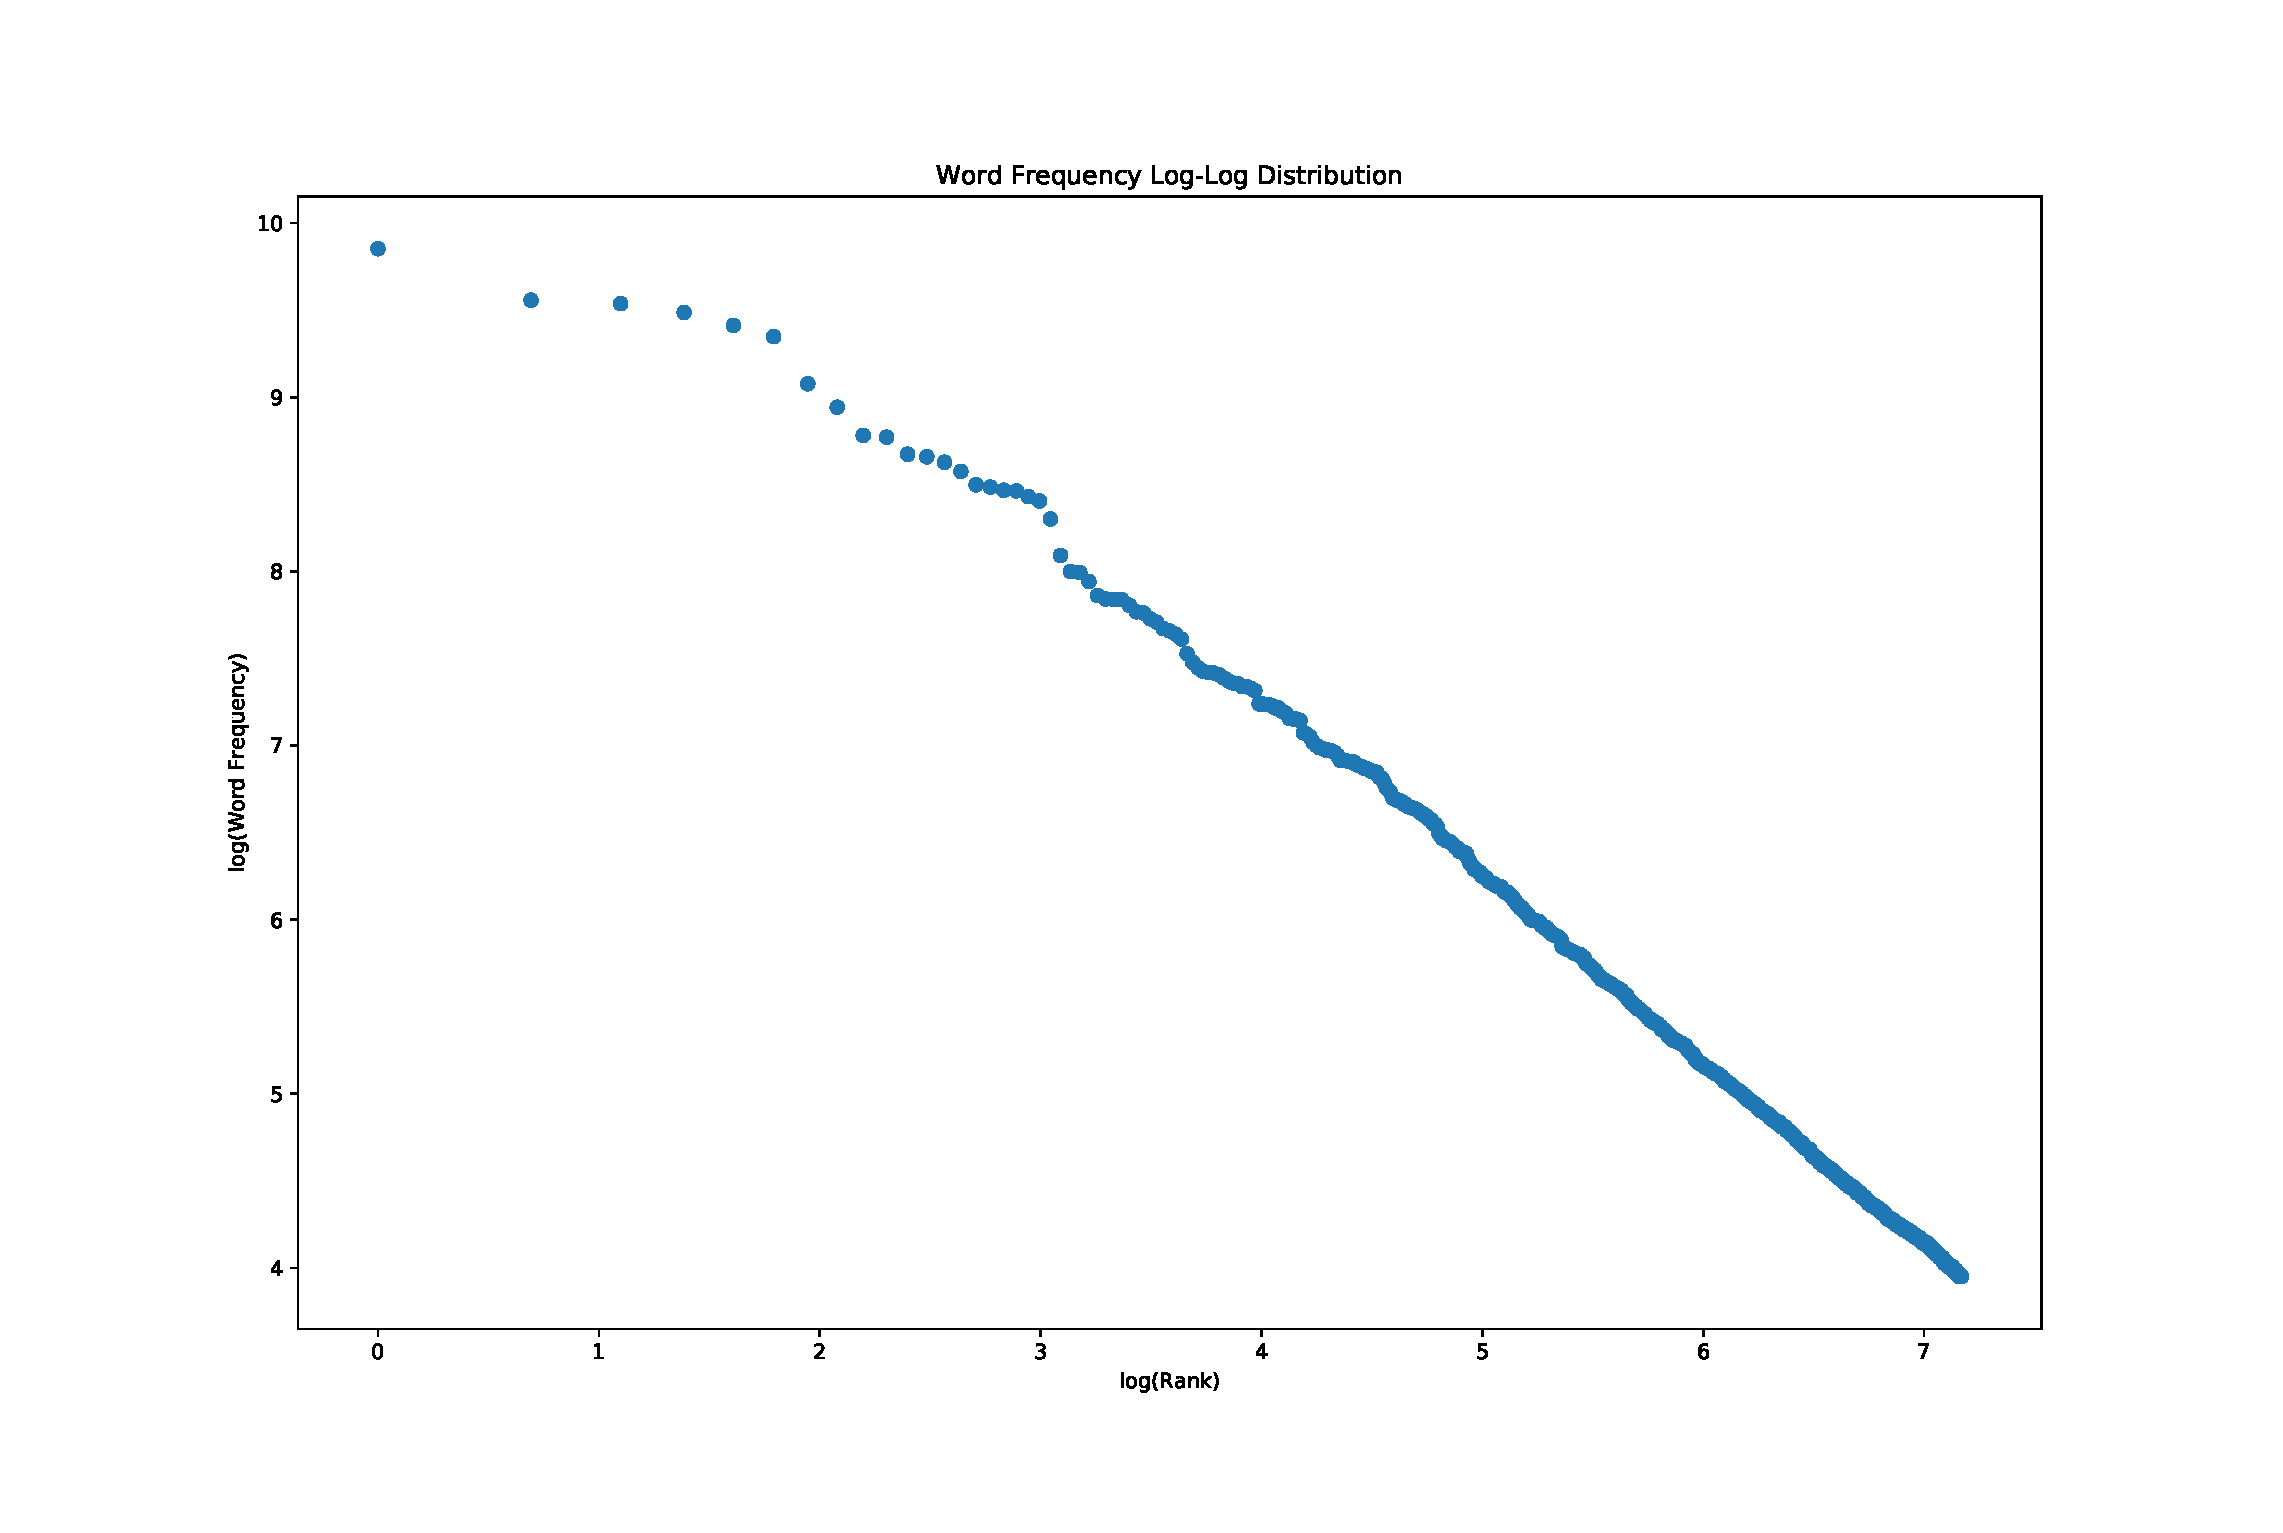
\includegraphics[scale=.25]{loglog_freq.eps}
\caption{Above is a scatterplot of the word frequencies plotted against rank transformed via log-log. This is done so we can check to see if the words follow Zipf's law. It does indeed seem to be that case (especially for low-frequency words) that it does follow a linear log-log distribution.
} \label{loglog_freq.eps}
\end{figure}

There has been growing interest in using and mitigating the use of social media in information warfare.~\cite{ref_lncs1} During and after the 2016 U.S. Presidential Election, multiple sources confirmed there had been a strong campaign to utilize social media to impact political views and partisanship.~\cite{ref_article1} We shall be examining some of the data from this campaign.
The data we will be looking at consists of Russian Troll Tweet data taken from accounts linked to the Internet Research Agency, or IRA. According to the U.S. Justice Department~\cite{ref_url1}, the IRA had direct links to the Russian Kremlin. Two researchers from Clemson University, Darren Linvill and Patrick Warren, mined the original data by using specialized software to identify and record tweets sent out by trolls linked to the IRA. FiveThirtyEight then received the data from the researchers.~\cite{ref_url4} These tweets were mixed with a large tweet set obtained from a 2009 paper on Twitter sentiment analysis.~\cite{ref_lncs2}



We were interested in what trolls are trying to affect and how they are achieving their goals. How could one try to decipher their goals? One simple methodology would be to look at word frequencies of troll tweets normalized via tf–idf (term frequency–inverse document frequency) to see which words tend to have the most weight.
We first cleaned the tweets by removing all stopwords and punctuation. Tweet specific punctuations such as \#, @ and emojis were kept.

~\\

Below shows how to compute the tf-idf; t = term, d = tweet, D = all tweets, N = total number of tweets, $n_t$ = number of occurrences of term t in all tweets.

\begin{align*}
\mathrm{tf}(t,d) = f_{t,d} \Bigg/ {\sum_{t' \in d}{f_{t',d}}} \\
\mathrm{idf}(t, D) = - \log \frac {n_t} {N} \\
\mathrm{tfidf}(t,d,D) = \mathrm{tf}(t,d) \cdot \mathrm{idf}(t, D)\\
\end{align*}

We then took the tf-idf matrix for each tweet, summed the the tweet matrices, and built a WordCloud based on the aggregate frequencies. This can be seen in Figure ~\ref{pre_cloud.eps}. 

\begin{figure}
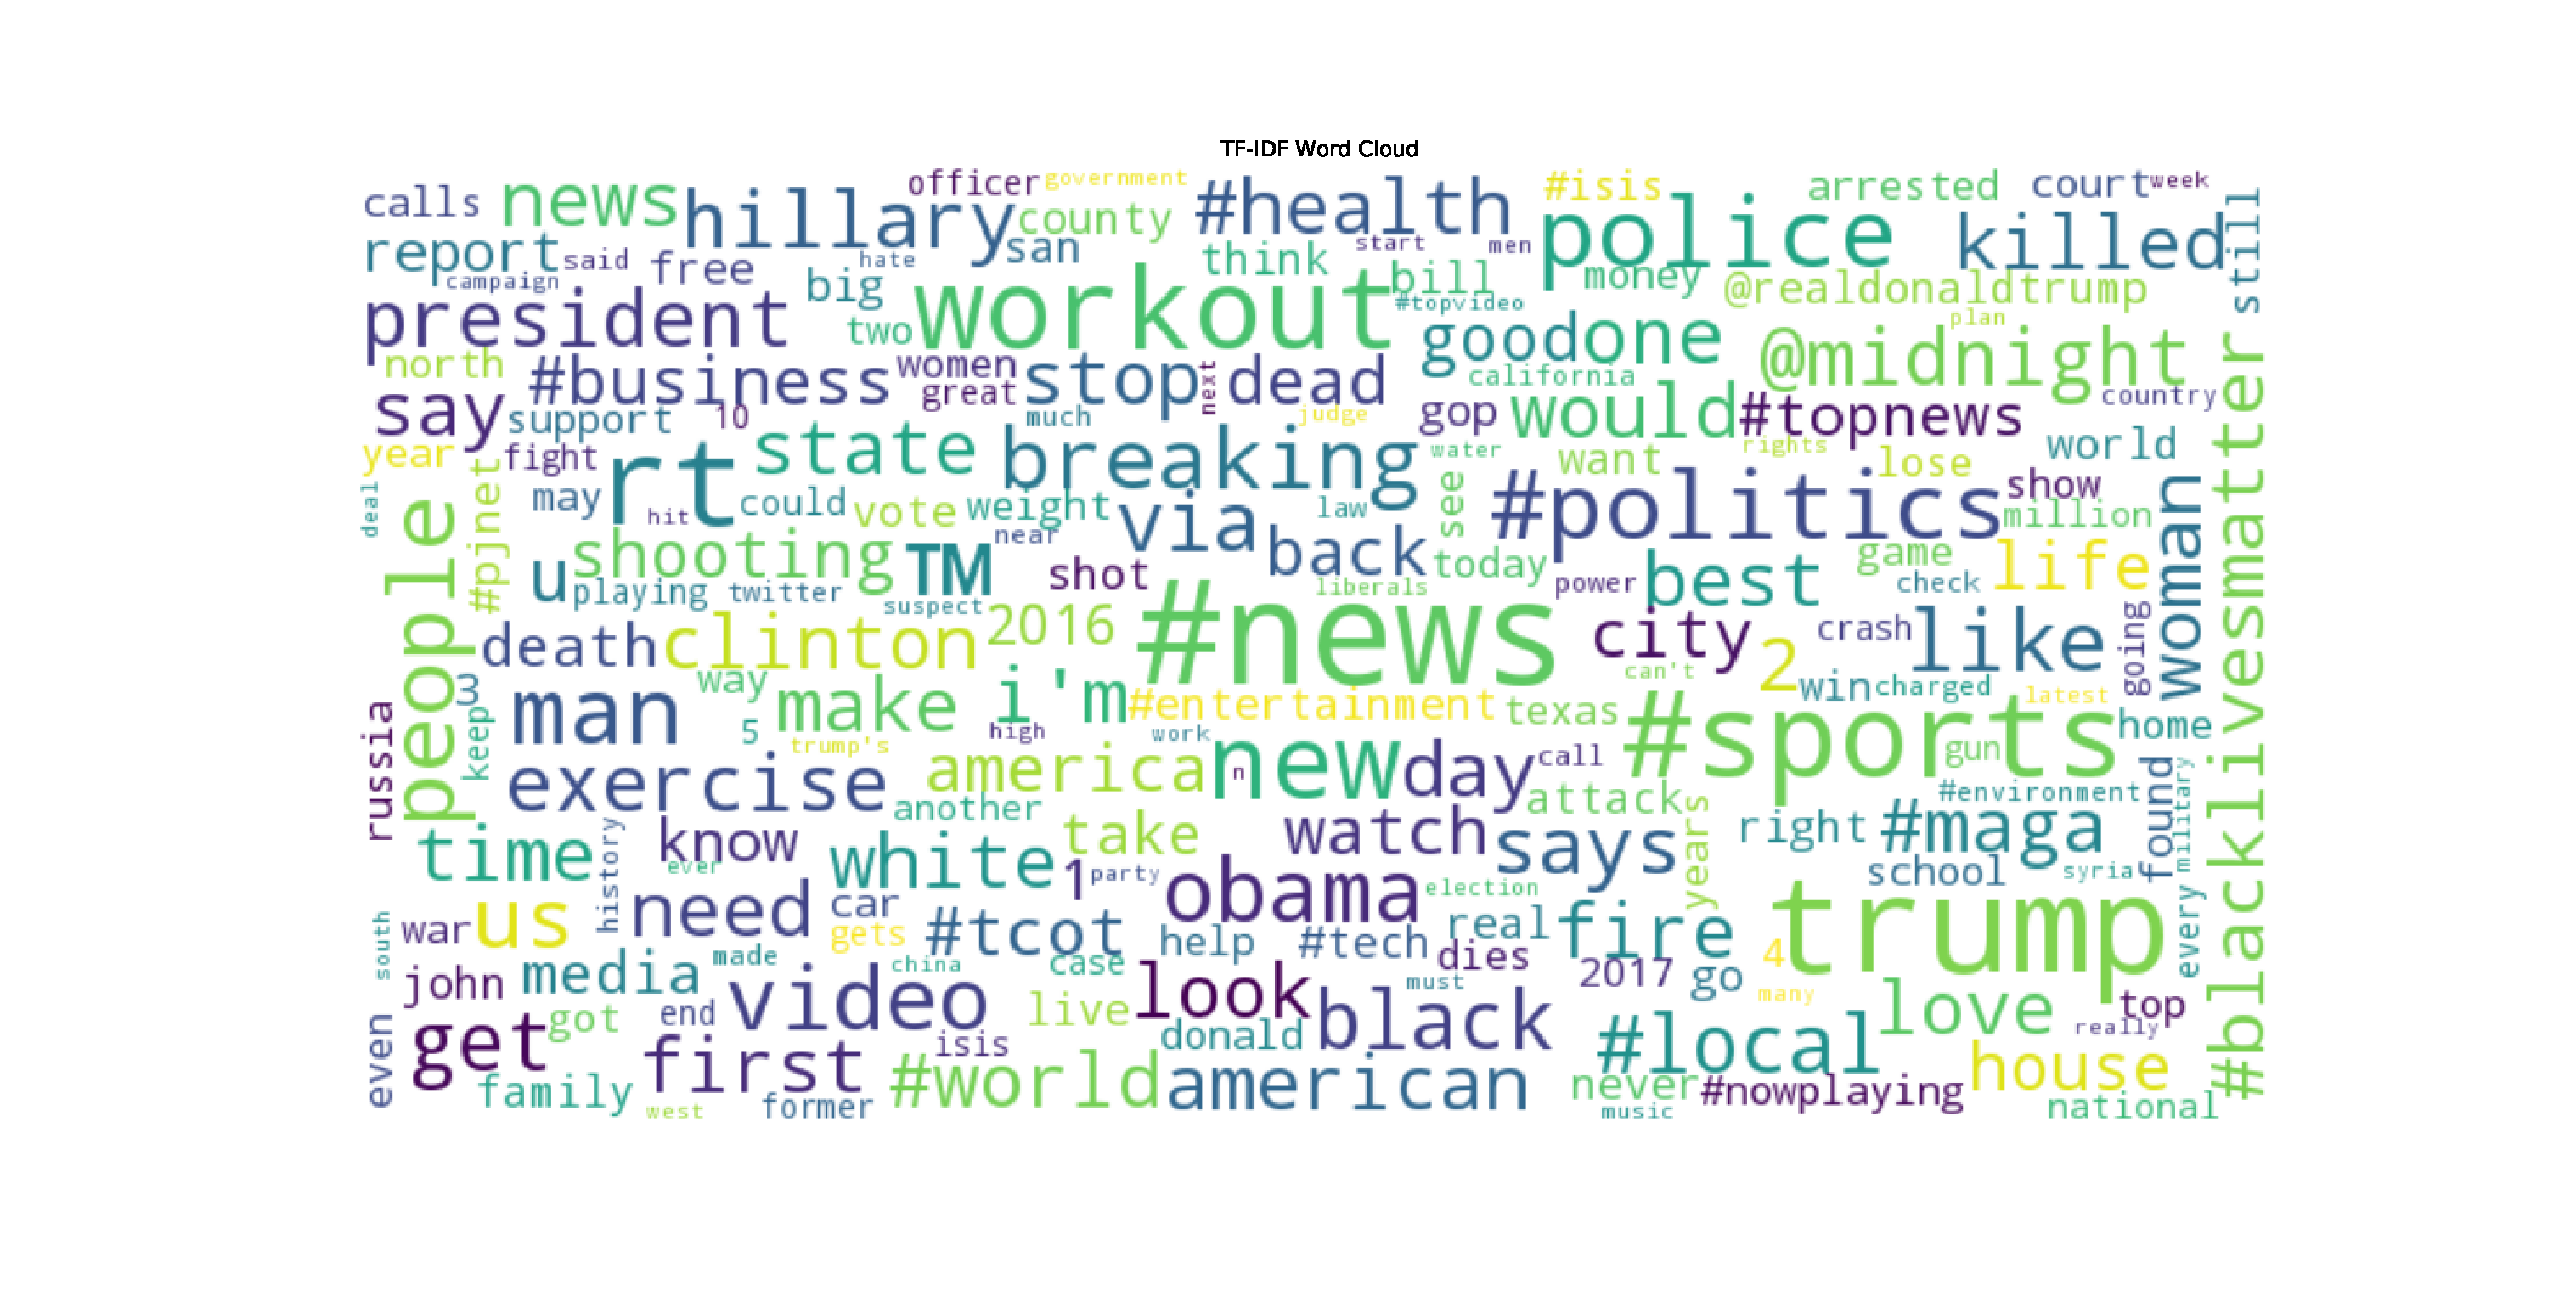
\includegraphics[width=\textwidth]{pre_cloud.eps}
\caption{This graph shows a WordCloud of the words with the greatest aggregate tf-idf. Note that this already tends to showcase many words which are uniquely identifying.} \label{pre_cloud.eps}
\end{figure}

\subsection{Logistic Regression}

Then we were interested in improving this analysis by introducing supervised learning. The main idea is that the words which the trained model gives the most (aggregate) weights are words which are most associated with a troll's information intentions. This may be an improvement over untrained raw tf-idf, because now we can separate what words are a detractor to troll tweets.
We will be using a simple binary logistic regression to classify each tweet as either troll or not troll by the TF-IDF or term frequency–inverse document frequency. We were not looking for the 'state of the art' solution to this supervised training problem. Given the historical nature of the data, we would not expect the prediction using any 'state of the art' system to remain constant.
\newline

We have a binary logistic regression model. Data is given as $D = {(\mathbf{x}_i, y_i):, i = 1...n}$, where $y_i \in \{-1, +1\}$, and $\mathbf{x}_i \in R^p$. In this case there are n samples and each sample has p features.

Let $ \mathbf{w'} =  \begin{bmatrix} b\\ \mathbf{w} \end{bmatrix}$ and $\mathbf{x}' = \begin{bmatrix} 1\\ \mathbf{x} \end{bmatrix}$. 
\begin{align*}
L(\mathbf{w'}) = \prod_{i=1}^{n} \frac{1}{1+exp\{-y(\mathbf{w'} \cdot \mathbf{x'_i})\}}\\
LL(\mathbf{w'}) = -\sum_i\log\{1+\exp\{-y_i(\mathbf{w'} \cdot \mathbf{x'_i})\}\}\\
PLL(\mathbf{w'}) = -\sum_i\log\{1+\exp\{-y_i(\mathbf{w'} \cdot \mathbf{x'_i})\}\}   - \frac{\alpha}{2}\sum_{j=1}^{p} w_j^2
\end{align*}
where j is between 0 and p (we don't sum j=0 in the $l^2$ penalty since $w_0=b$).
\newline

We can then find our optimal weights using gradient decent. Below is the gradient needed to implement the update.

\begin{align*}
\nabla PLL(\mathbf{w'}) = -\sum_i\frac{-y_i}{1+\exp\{-y_i(\mathbf{w'}\cdot \mathbf{x'_i})\}}\begin{bmatrix} \exp\{-y_i(\mathbf{w'}\cdot\mathbf{x'_i})\} \\ (x_1)\exp\{-y_i(\mathbf{w'}\cdot\mathbf{x'_i})\}\\ \vdots \\ (x_p)\exp\{-y_i(\mathbf{w'}\cdot\mathbf{x'_i})\}\\ \end{bmatrix} - \begin{bmatrix} 0 \\ \alpha(w_1) \\ \vdots \\ \alpha(w_p) \\ \end{bmatrix}
\end{align*}
 
We can then implement the gradient decent. The specific code is in the included jupyter notebook.
Now we can train our data. The csv file contained 200,000 tweets but only 60,000 were used; 45,000 for training and 15,000 for testing.  The training size was smaller than expected for a few different reasons. The main reason was when we used more training sets, validation error (error when comparing our prediction with the two outside tweet sets) tended to increase. Computational complexity was also taken into consideration. Through trial and error, we found that an $\alpha=-1500$ was most effective, yes with the negative alpha (an unbounded log likelihood). When we did have positive regularization (or no regularization), we found the bounded log likelihood would be fine for our training and test data (they were always around 83\% accuracy within .5\% of each other) but the other 'unknown' tweet sets tended to perform significantly worse. Future work could implement an $l^1$ regularization to see if this helps make regularization (in the 'correct' direction) useful.
\begin{figure}
\centering
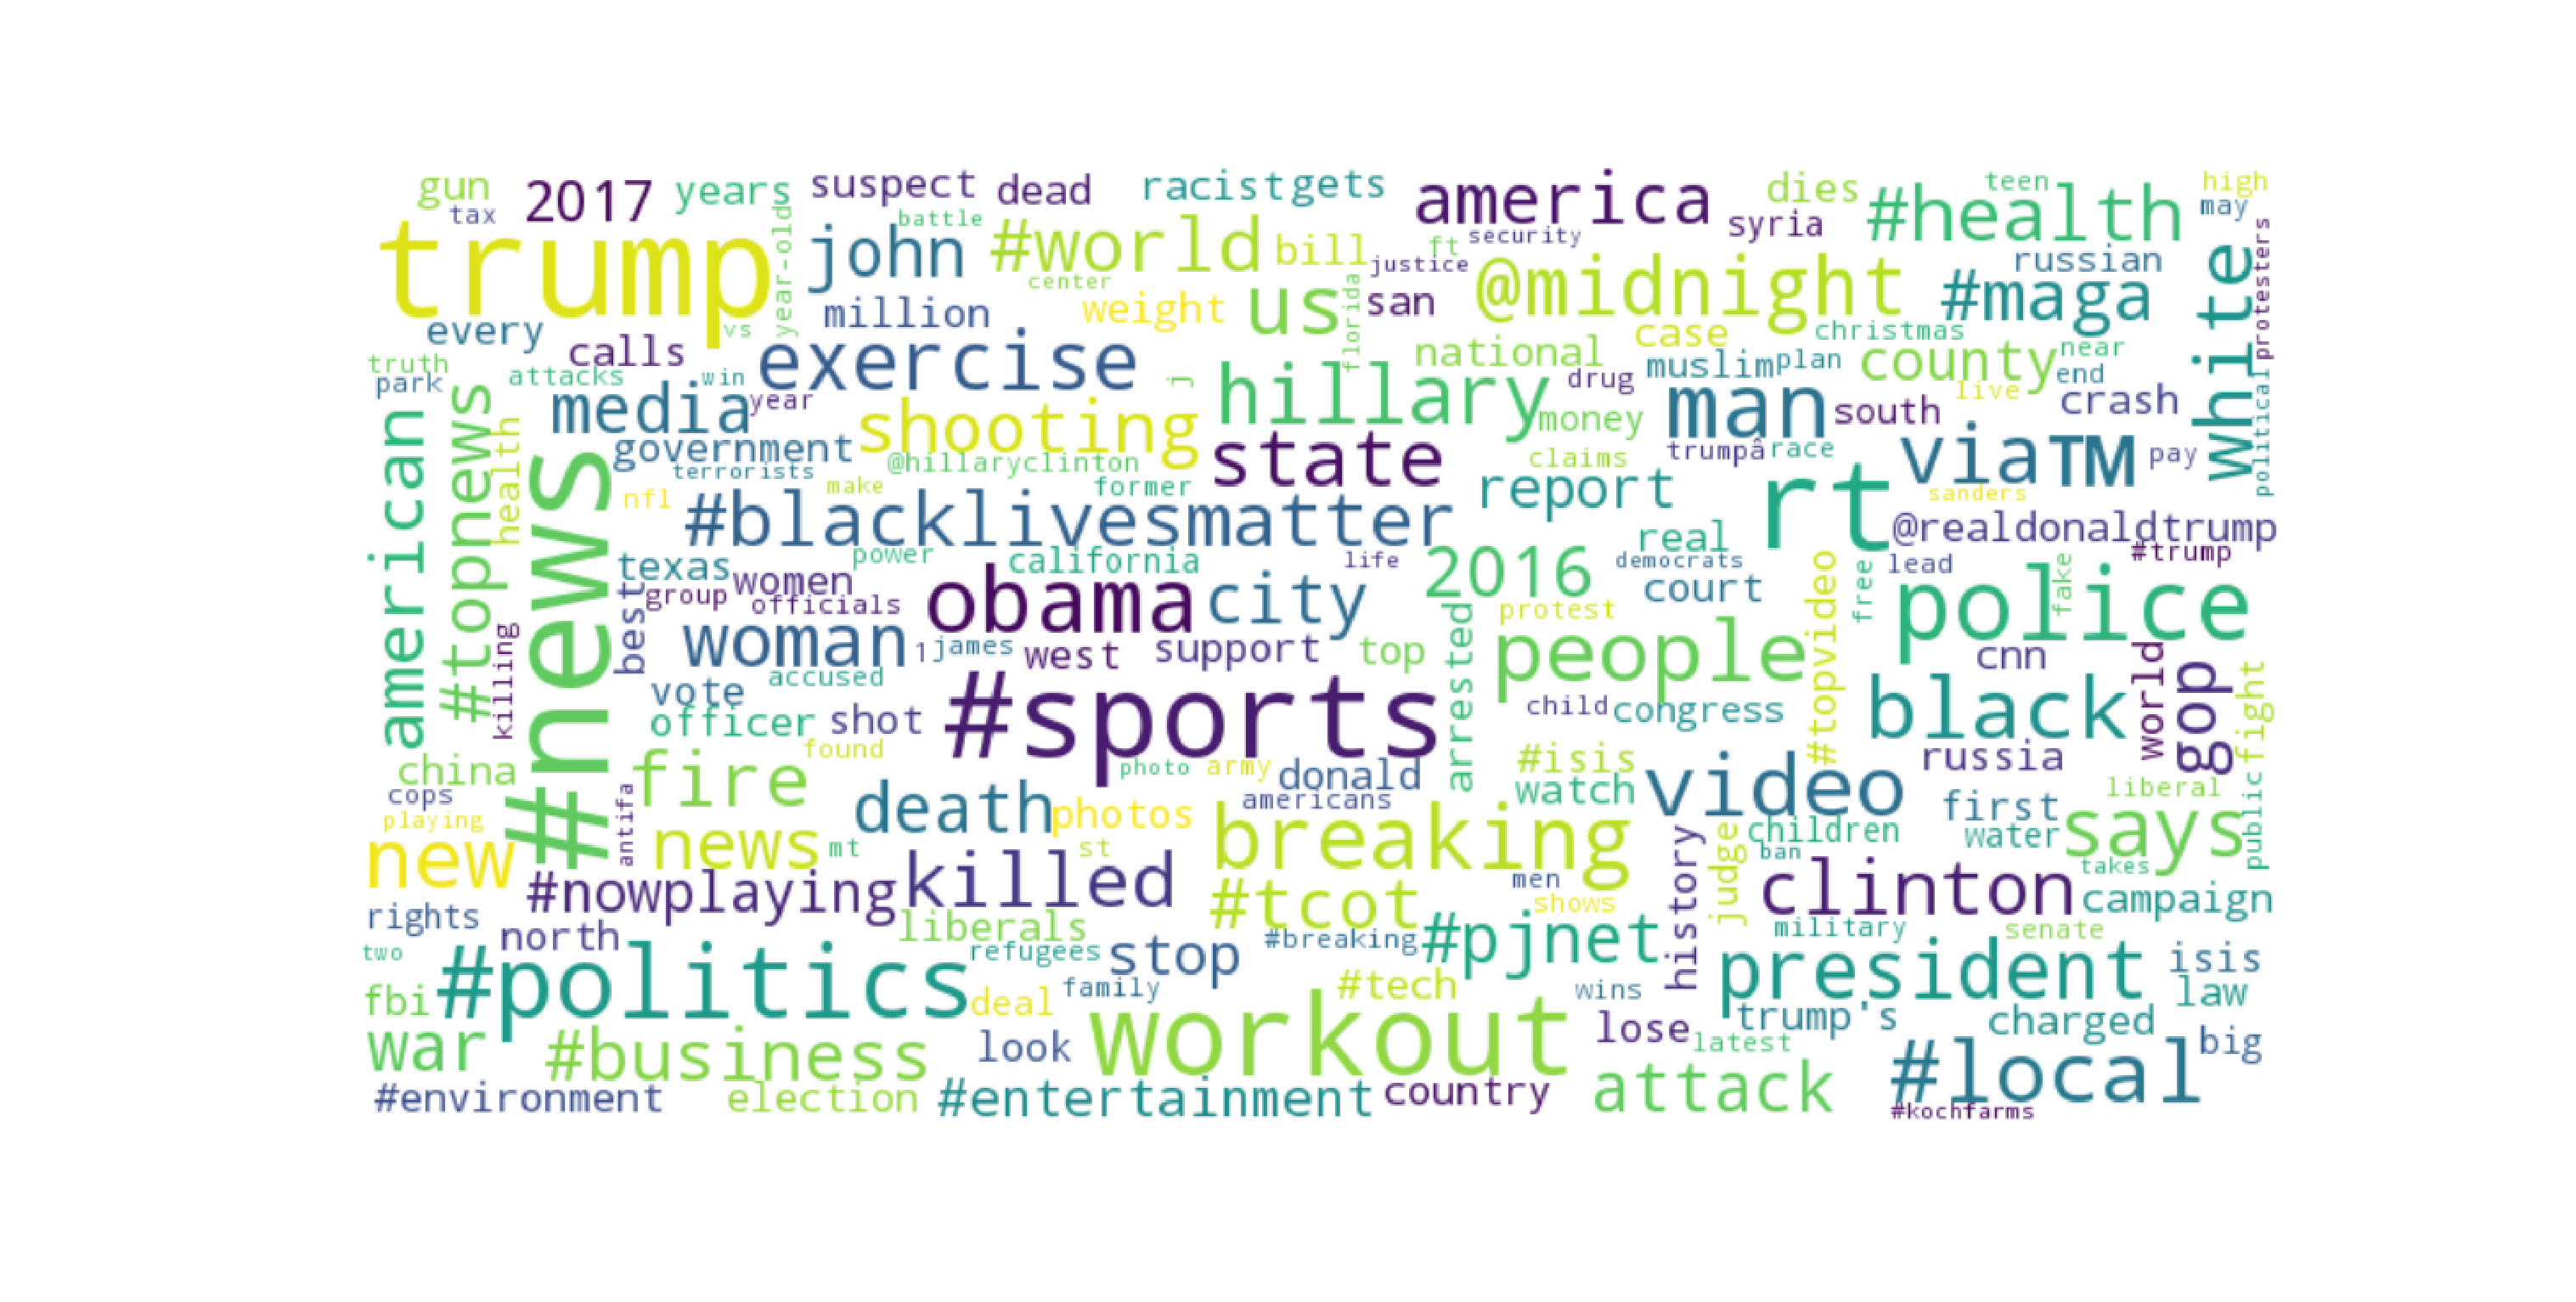
\includegraphics[width=\textwidth]{test_troll.eps}
\caption{This WordCloud shows the words with greatest impact (aggregate TF-IDF multiplied by their training weights) for tweets in the test dataset which were predicted correctly and that were troll tweets.
} \label{test_troll.eps}
\end{figure}
We ran our gradient decent optimization for a total of 600 iterations and obtained a training accuracy of 83.6\% and a test accuracy of 83.2\%.
Our main interest was to see if, after the training weights were optimized, we could extract useful word features from the trolls that could tell us more about their objectives goals. As before we will sum up all the TF-IDF matrices, but they are now weighted post training (with our learned weights). We then rank the words which had the highest scores with weights and produce a WordCloud. Figure ~\ref{test_troll.eps} shows us these most important words and that they have a striking similarity to the pre-trained TF-IDF WordCloud. The figure shows many strong political words and hashtags as before. Unfortunately, it appears that our desire to obtain additional information on the 'intention' of the troll users has not been effective with this method. However, this outcome does reinforce the confidence that these words are indeed quite reflective of troll intention. This paints a picture similar to the official 'Western' narratives previously cited.~\cite{ref_article1}~\cite{ref_url1}


\section{Additional Datasets}
We now bring in two outside Twitter datasets ~\cite{ref_url2}~\cite{ref_url3} (which we intentionally did not include any portion in our training model) to assess the effectiveness of our model. The first is a dataset only consisting of tweets related to airline companies (mostly people tweeting complaints) and the second is a set containing tweets related to the first 2016 GOP debate. Each dataset only contained tweets coded as non-trolls.
We obtained an accuracy of 78.3\% for the airline tweets, but only an accuracy of 22.0\% for the GOP debate tweets. It is likely that our model over-fits with respect to strong political tweets. It may be less of a troll predictor and more of a political tweet predictor. This would make sense considering the most important words we found for predicting a troll were generally political tweets (which is in alignment with the known intentions of the trolls).

\section{Future Work}
This biggest issues with this work were the lack of obtaining additional high-value words after training and the poor predictive performance of the GOP debate tweets. More advanced models, such as SVMs, could help address this issue. Word ngrams, such as bigrams or trigrams, could also be used. This way we could consider more complex word patterns, which may help surface more direct troll intentions (and make the prediction model more effective).



%
% ---- Bibliography ----
%
% BibTeX users should specify bibliography style 'splncs04'.
% References will then be sorted and formatted in the correct style.
%
% \bibliographystyle{splncs04}
% \bibliography{mybibliography}
%
\begin{thebibliography}{8}

\bibitem{ref_url2}
Figure Eight, Airline Twitter Sentiment, Version 2. Retrieved 15 Nov 2018 from \url{https://www.kaggle.com/crowdflower/twitter-airline-sentiment/downloads/twitter-airline-sentiment.zip/2}. (2015, February).

\bibitem{ref_url3}
Figure Eight, First GOP debate sentiment analysis, Version 1. Retrieved 20 Nov 2018 from \url{https://www.kaggle.com/crowdflower/first-gop-debate-twitter-sentiment/downloads/first-gop-debate-twitter-sentiment.zip/2}. (2015, August).

\bibitem{ref_url4}
FiveThirtyEight, Russian Troll Tweets, GitHub repository, \url{https://github.com/fivethirtyeight/russian-troll-tweets}. (2018).


\bibitem{ref_lncs2}
Go, A., Bhayani, R. and Huang, L., 2009. Twitter sentiment classification using distant supervision. CS224N Project Report, Stanford, 1(2009), p.12.

\bibitem{ref_lncs1}
Griffin, C., Bickel, B. Unsupervised Machine Learning of Open Source Russian Twitter Data Reveals Global Scope and Operational Characteristics. arXiv preprint arXiv:1810.01466. (2018).

\bibitem{ref_article1}
National Intelligence Council (U.S.), “Assessing Russian activities and intentions in recent US elections,” Office of the Director of National Intelligence, National Intelligence Council, Washington, D.C., 2017.

\bibitem{ref_url1}
US Department of Justice News, \url{https://www.justice.gov/opa/pr/grand-jury-indicts-thirteen-russian-individuals-and-three-russian-companies-scheme-interfere}. Last accessed 9 Dec 2018





\end{thebibliography}
\end{document}
